%%%%%%%%%%%%%%%%%%%%%%%%%%%%%%%%%%%%%%%%%%%%%%%%%%%%%%%%%%%%%%%%
%%                                                            %%
%%   essentialsOfLatin, Italian translation 2017              %%
%%                                                            %%
%% From:  Henry C. Pearson, Essentials Of Latin For Beginners %%
%%        (1915, New York, American Book Company)             %%
%%                                                            %%
%%    https://archive.org/details/essentialslatin04peargoog   %%
%%                                                            %%
%% Translated by g.p.ciceri <gp.ciceri@gmail.com>             %%
%% ---------------------------------------------------------- %%
%% This translation is Licensed under                         %%
%% Creative Commons Attribution-ShareAlike 4.0 International  %%
%% https://creativecommons.org/licenses/by-sa/4.0/            %%
%%                                                            %%
%%%%%%%%%%%%%%%%%%%%%%%%%%%%%%%%%%%%%%%%%%%%%%%%%%%%%%%%%%%%%%%%

% āēīōū
% ăĕĭŏŭ




\documentclass[nols]{tufte-handout}

%\geometry{showframe} % display margins for debugging page layout

\usepackage{fontspec}
\usepackage{ifxetex}
\setmainfont[Path=./fonts/palatino-linotype/, ItalicFont=palai.ttf, BoldFont=palab.ttf]{pala.ttf}


% \defaultfontfeatures{Mapping=tex-text}
% \setromanfont[Path=./fonts/TeX-Gyre-Schola/,Mapping=tex-text]{TeX Gyre Schola}
% \setsansfont[Path=./fonts/TeX-Gyre-Heros/,Scale=MatchLowercase,Mapping=tex-text]{TeX Gyre Heros}
% \setmonofont[Path=./fonts/TeX-Gyre-Cursor/,Scale=MatchLowercase]{TeX Gyre Cursor}

\usepackage{lipsum}
\usepackage{url}
\usepackage{longtable}
\usepackage{stackengine}

\usepackage{graphicx} % allow embedded images
  \setkeys{Gin}{width=\linewidth,totalheight=\textheight,keepaspectratio}
  \graphicspath{{graphics/}} % set of paths to search for images
\usepackage{amsmath}  % extended mathematics
\usepackage{booktabs} % book-quality tables
\usepackage{units}    % non-stacked fractions and better unit spacing
\usepackage{multicol} % multiple column layout facilities
\usepackage{lipsum}   % filler text
\usepackage{fancyvrb} % extended verbatim environments
  \fvset{fontsize=\normalsize}% default font size for fancy-verbatim environments

% Standardize command font styles and environments
\newcommand{\doccmd}[1]{\texttt{\textbackslash#1}}% command name -- adds backslash automatically
\newcommand{\docopt}[1]{\ensuremath{\langle}\textrm{\textit{#1}}\ensuremath{\rangle}}% optional command argument
\newcommand{\docarg}[1]{\textrm{\textit{#1}}}% (required) command argument
\newcommand{\docenv}[1]{\textsf{#1}}% environment name
\newcommand{\docpkg}[1]{\texttt{#1}}% package name
\newcommand{\doccls}[1]{\texttt{#1}}% document class name
\newcommand{\docclsopt}[1]{\texttt{#1}}% document class option name
\newenvironment{docspec}{\begin{quote}\noindent}{\end{quote}}% command specification environment

% concetti morfosintattici
\usepackage{xspace} 
\newcommand{\noun}{\textsc{sostantivo}\xspace}
\newcommand{\nouns}{\textsc{sostantivi}\xspace}
\newcommand{\adject}{\textsc{aggettivo}\xspace}
\newcommand{\adjects}{\textsc{aggettivi}\xspace}
\newcommand{\gnumber}{\textsc{numero}\xspace}
\newcommand{\gnumbers}{\textsc{numeri}\xspace}
\newcommand{\gender}{\textsc{genere}\xspace}
\newcommand{\genders}{\textsc{generi}\xspace}
\newcommand{\gcase}{\textsc{caso}\xspace}
\newcommand{\gcases}{\textsc{casi}\xspace}
\newcommand{\tense}{\textsc{tempo}\xspace}
\newcommand{\mood}{\textsc{modo}\xspace}
\newcommand{\gverb}{\textsc{verbo}\xspace}
\newcommand{\gverbs}{\textsc{verbi}\xspace}
\newcommand{\adjective}{\textsc{aggettivo}\xspace}
\newcommand{\nom}{\textsc{nom}\xspace}
\newcommand{\gen}{\textsc{gen}\xspace}
\newcommand{\dat}{\textsc{dat}\xspace}
\newcommand{\acc}{\textsc{acc}\xspace}
\newcommand{\voc}{\textsc{voc}\xspace}
\newcommand{\abl}{\textsc{abl}\xspace}
\newcommand{\gexit}{\textsc{uscita}\xspace}
\newcommand{\gexits}{\textsc{uscite}\xspace}
\newcommand{\declinazione}{\textsc{declinazione}\xspace}
\newcommand{\masc}{\textsc{maschile}\xspace}
\newcommand{\femm}{\textsc{femminile}\xspace}
\newcommand{\neut}{\textsc{neutro}\xspace}

\newcommand{\indic}{\textsc{indicativo}\xspace}
\newcommand{\imper}{\textsc{imperativo}\xspace}
\newcommand{\gcong}{\textsc{congiuntivo}\xspace}
\newcommand{\ott}{\textsc{ottativo}\xspace}
\newcommand{\partic}{\textsc{participio}\xspace}
\newcommand{\infin}{\textsc{infinito}\xspace}

\newcommand{\pres}{\textsc{presente}\xspace}
\newcommand{\imperf}{\textsc{imperfetto}\xspace}
\newcommand{\aor}{\textsc{aoristo}\xspace}
\newcommand{\fut}{\textsc{futuro}\xspace}
\newcommand{\perf}{\textsc{perfetto}\xspace}
\newcommand{\pperf}{\textsc{piuccheperfetto}\xspace}

\newcommand{\sing}{\textsc{singolare}\xspace}
\newcommand{\plur}{\textsc{plurale}\xspace}
\newcommand{\dual}{\textsc{duale}\xspace}

\newcommand{\si}{\textsc{sing}\xspace}
\newcommand{\pl}{\textsc{plur}\xspace}
\newcommand{\du}{\textsc{dual}\xspace}

\newcommand{\att}{\textsc{attivo}\xspace}
\newcommand{\med}{\textsc{medio}\xspace}
\newcommand{\pass}{\textsc{passivo}\xspace}
\newcommand{\medpass}{\textsc{medio-passivo}\xspace}


% italianitudini
\renewcommand{\figurename}{Figura}
\renewcommand{\tablename}{Tabella}
\renewcommand{\contentsname}{Indice}

% fix per un qualche problema
\ifxetex
  \newcommand{\textls}[2][5]{%
    \begingroup\addfontfeatures{LetterSpace=#1}#2\endgroup
  }
  \renewcommand{\allcapsspacing}[1]{\textls[15]{#1}}
  \renewcommand{\smallcapsspacing}[1]{\textls[10]{#1}}
  \renewcommand{\allcaps}[1]{\textls[15]{\MakeTextUppercase{#1}}}
  \renewcommand{\smallcaps}[1]{\smallcapsspacing{\scshape\MakeTextLowercase{#1}}}
  \renewcommand{\textsc}[1]{\smallcapsspacing{\textsmallcaps{#1}}}
\fi

% too many float...
\extrafloats{100}

\title{Essentials Of Latin. Elementi di Latino. \newline Lezione XXIV - Aggettivi della Seconda Classe a Due e Una Uscita. Dativo con Aggettivi.}

\author[gpciceri]{a cura di Milagathòs: Milo's help to enjoy humanities.}

\date{26 Febbrajo 2017} % without \date command, current date is supplied


\begin{document}

\hyphenation{co-niu-ga-zio-ne}

\maketitle% this prints the handout title, author, and date

\begin{marginfigure}[-2.5cm]
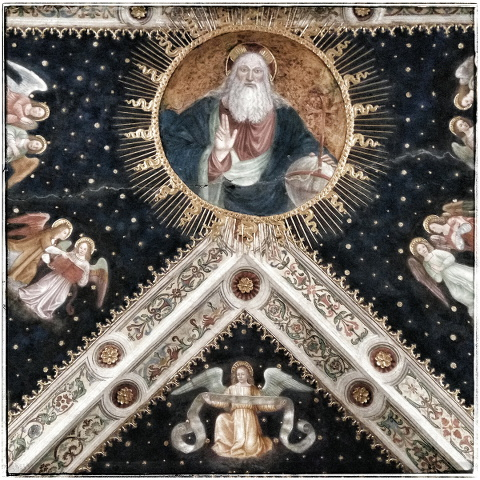
\includegraphics{smallthumb-lesson_XI.jpeg}
\setfloatalignment{b}
\end{marginfigure}


\begin{abstract}
\noindent
Queste lezioni riprendono il testo introduttivo al Latino di Pearson\cite{pearson1915}, del quale seguono la numerazione; la struttura di ogni lezione è piuttosto regolare: inizia con \textsc{cenni di morfologia e di sintassi latina}, seguita da un \textsc{piccolo vocabolario} per il lessico; ci sono infine vari \textsc{esercizi} di traduzione e di composizione latina.

\bigskip
\noindent
Lezione XXIV - Aggettivi della Seconda Classe a Due e Una Uscita. Dativo con Aggettivi. Vocabolario, esercizi.
\end{abstract}

%\printclassoptions

\newthought{161.} Molti aggettivi della Seconda Classe hanno solo due forme distinte al nominativo singolare, una per il maschile e il femminile ed un'altra per il neutro. Tranne che per i comparativi (vedi poi (257.)) sono tutti declinati allo stesso modo:

% āēīōū
% ăĕĭŏŭ

\begin{fullwidth}
\begin{table}[!htbp]
  \centering
  \begin{tabular}{l l l l}
    %\toprule
	\multicolumn{4}{c}{\textbf{facilis}, \textit{semplice, facile}} \\
	\multicolumn{4}{c}{\textsc{Tema} \textbf{facili-}, \textsc{Radice} \textbf{facil-}} \\
	
	\multicolumn{4}{c}{\textsc{Singolare}} \\
	& \multicolumn{1}{c}{\textsc{Maschile e Femminile}} & \hspace{20mm} & \multicolumn{1}{c}{\textsc{Neutro}} \\
	
    \textsc{Nom.} & facil\textbf{is} & & facil\textbf{e} \\
    \textsc{Gen.} & facil\textbf{is} & & facil\textbf{is} \\
    \textsc{Dat.} & facil\textbf{ī} & & facil\textbf{ī} \\
    \textsc{Acc.} & facil\textbf{em} & & facil\textbf{e} \\
    \textsc{Voc.} & facil\textbf{is} & & facil\textbf{e} \\
    \textsc{Abl.} & facil\textbf{ī} & & facil\textbf{ī} \\
	
	\multicolumn{4}{c}{\textsc{Plurale}} \\
	
    \textsc{Nom.} & facil\textbf{ēs} & & facil\textbf{ia} \\
    \textsc{Gen.} & facil\textbf{ium} & & facil\textbf{ium} \\
    \textsc{Dat.} & facil\textbf{ibus} & & facil\textbf{ibus} \\
    \textsc{Acc.} & facil\textbf{īs (ēs)} & & facil\textbf{ia} \\
    \textsc{Voc.} & facil\textbf{ēs} & & facil\textbf{ia} \\
    \textsc{Abl.} & facil\textbf{ibus} & & facil\textbf{ibus} \\
    
    %\bottomrule
  \end{tabular}
  %\caption{}
  \label{tab:normaltab}
  %\zsavepos{pos:normaltab}
\end{table}
\end{fullwidth}

\newthought{} Altri aggettivi della Seconda Classe hanno una sola forma per il nominativo singolare, valida per tutti i generi. Si declinano come:

% āēīōū
% ăĕĭŏŭ

\begin{fullwidth}
\begin{table}[!htbp]
  \centering
  \begin{tabular}{l l l l}
    %\toprule
	\multicolumn{4}{c}{\textbf{audax}, \textit{audace, coraggioso}} \\
	\multicolumn{4}{c}{\textsc{Tema} \textbf{audāci-}, \textsc{Radice} \textbf{audāc-}} \\
	
	\multicolumn{4}{c}{\textsc{Singolare}} \\
	& \multicolumn{1}{c}{\textsc{Maschile e Femminile}} & \hspace{20mm} & \multicolumn{1}{c}{\textsc{Neutro}} \\
	
    \textsc{Nom.} & audāx & & audāx \\
    \textsc{Gen.} & audāc\textbf{is} & & audāc\textbf{is} \\
    \textsc{Dat.} & audāc\textbf{ī} & & audāc\textbf{ī} \\
    \textsc{Acc.} & audāc\textbf{em} & & audāc\textbf{e} \\
    \textsc{Voc.} & audāx & & audāx \\
    \textsc{Abl.} & audāc\textbf{ī} & & audāc\textbf{ī} \\
	
	\multicolumn{4}{c}{\textsc{Plurale}} \\
	
    \textsc{Nom.} & audāc\textbf{ēs} & & audāc\textbf{ia} \\
    \textsc{Gen.} & audāc\textbf{ium} & & audāc\textbf{ium} \\
    \textsc{Dat.} & audāc\textbf{ibus} & & audāc\textbf{ibus} \\
    \textsc{Acc.} & audāc\textbf{īs (ēs)} & & audāc\textbf{ia} \\
    \textsc{Voc.} & audāc\textbf{ēs} & & audāc\textbf{ia} \\
    \textsc{Abl.} & audāc\textbf{ibus} & & audāc\textbf{ibus} \\
    
    %\bottomrule
  \end{tabular}
  %\caption{}
  \label{tab:normaltab}
  %\zsavepos{pos:normaltab}
\end{table}
\end{fullwidth}


\newthought{Osservazioni}
\begin{itemize}
\item[\textsc{1.}] Tutti gli aggettivi della Seconda Classe hanno una sola forma per tutti i generi in tutti i casi, eccetto il \nom e l'\acc.  
\item[\textsc{1.}] Gli aggettivi della Seconda classe che terminao in \textbf{-er} hanno tre uscite, quelli in \textbf{-is} due e tutti gli altri (eccetto i comparativi) una.  
\item[\textsc{1.}] Tutti gli aggettivi della Seconda Classe hanno il tema in \textbf{-i-}, quelli a tre o a due uscite hanno solo \textbf{-ī} all'ablativo singolare.  
\end{itemize}

\newthought{162. Frasi Modello.} Esamina le seguenti frasi:
\begin{itemize}
\item[\textsc{1.}] \textbf{Filius patri similis erat}, \textit{il figlio era simile al padre}.  
\item[\textsc{2.}] \textbf{Locus castris idoneus erat}, \textit{il luogo era idoneo all'accampamento}.  
\end{itemize}

Osserva che i dativi \textbf{patri, castris} sono collegati agli aggettivi \textbf{similis, idoneus}. 

\newthought{163. Regola \textemdash Dativo con gli Aggettivi.} Con aggettivi che significano somiglianza, idoneità, vicinanza, servizio, inclinazione e con i loro opposti si usa il dativo per il termine indicato.

% āēīōū
% ăĕĭŏŭ

\newthought{164. Vocabolario}

\begin{multicols}{2}
    \noindent \hangindent=1em \textbf{fortis, -e}, agg., \textit{forte, coraggioso}.  \\
	\noindent \hangindent=1em \textbf{similis, -e}, agg., \textit{somigliante, simile}.  \\
	\noindent \hangindent=1em \textbf{dissimilis, -e}, agg., \textit{dissimile, non somigliante}.  \\
	\noindent \hangindent=1em \textbf{facilis, -e}, agg., \textit{facile}.  \\
	\noindent \hangindent=1em \textbf{difficilis, -ee}, agg., \textit{difficile}.  \\
	\noindent \hangindent=1em \textbf{omnis, -e}, agg., \textit{tutto, ogni, intero}.  \\
    \noindent \hangindent=1em \textbf{brevis, -e}, agg., \textit{corto, breve}.  \\
    \noindent \hangindent=1em \textbf{par, paris}, agg., \textit{uguale}.  \\
    \noindent \hangindent=1em \textbf{vetus, veteris} (abl. \textbf{vetere}), agg., \textit{vecchio, antico}.  \\
    \noindent \hangindent=1em \textbf{gens, gentis}, f., \textit{razza, nazione}.  \\
    \noindent \hangindent=1em \textbf{populus, -i}, m., \textit{gente}. 
\end{multicols}


\newthought{165. Esercizi di Ripasso}
\\
\textsc{I.} \quad
\textsc{1.}~Helvetii fluminibus altis continebantur. \quad
\textsc{2.}~Ad flumen iter angustum erat. \quad
\textsc{3.}~Cur finitimi nostri terrentur? Quod cum Romanis pacem et amicitiam confirmivimus. \quad
\textsc{4.}~Caesar equestribus proeliis Gallos superavit. \quad
\textsc{5.}~Pedites nostri altis fluminibus terrebantur. \quad
\textsc{6.}~Gallos magna cum celeritate in fugam dederunt. \quad
\\
\textsc{II.} \quad
\textsc{1.}~Vi erano molte belle navi sul mare. \quad
\textsc{2.}~La nostra cavalleria era fiera in battaglia. \quad
\textsc{3.}~Perché erano spaventati? \quad
\textsc{4.}~I ponti erano stati presi dai nemici.

\newthought{166. Esercizi}
\\
\textsc{I.} \quad
\textsc{1.}~Multae et fortes erant in Gallia gentes. \quad
\textsc{2.}~Caesar veteres milites amabat, quod bello fortes erant. \quad
\textsc{3.}~Milites fortes oppidum occupaverant. \quad
\textsc{4.}~Iter ad montem facile est. \quad
\textsc{5.}~Brevi tempore magnam hostium partem necaverant. \quad
\textsc{6.}~Helvetii multitudine hominum populo Romani non erant pares. \quad
\textsc{7.}~Puer fortis a milite vulneratus est. \quad
\textsc{8.}~Omnes incolae ex oppido ad collem convocantur. \quad
\textsc{9.}~Caesar multis imperatoribus dissimilis erat. \quad
\textsc{10.}~Finitimi nostri omnes gentes virtute superant. 
\\
\textsc{II.} \quad
\textsc{1.}~Vedremo molti bambini in ogni città. \quad
\textsc{2.}~Il ragazzo era come la ragazza in dimensioni \quad
\textsc{3.}~Portammo il grano in città per una strada facile. \quad
\textsc{4.}~Tutte le tribù erano coraggiose e fedeli. \quad
\textsc{5.}~In Inverno i cami vicino al fiume non erano adatti per un accampamento. \quad
\textsc{6.}~Il popolo Romano non fu conquistato dai coraggiosi Elvezi.

\newthought{(448.) Lettura. I Romani e gli elefanti}
Pyrrhum, Epiri regem, quod fortis vir bonusque imperator erat, Tarenti cives in Italiam vocaverunt. 
Cum Romanis multis proeliis dimicavit Romanesque superavit, quod elephantos in Italiam portaverat, quae animalia 
ante Pyrrhi tempus a Romanis non visa erant. 
Sed Romani, viri audaces, pedes elephantorum pilis vulnerabant magnaque animalium caedes fuit. 
Pari virtute milites cum Pyrrhi copiis dimicaverunt. 
Omnia corpora necatorum Romanorum vulnera in capitibus habuerunt. 

\begin{figure}[!b]
  %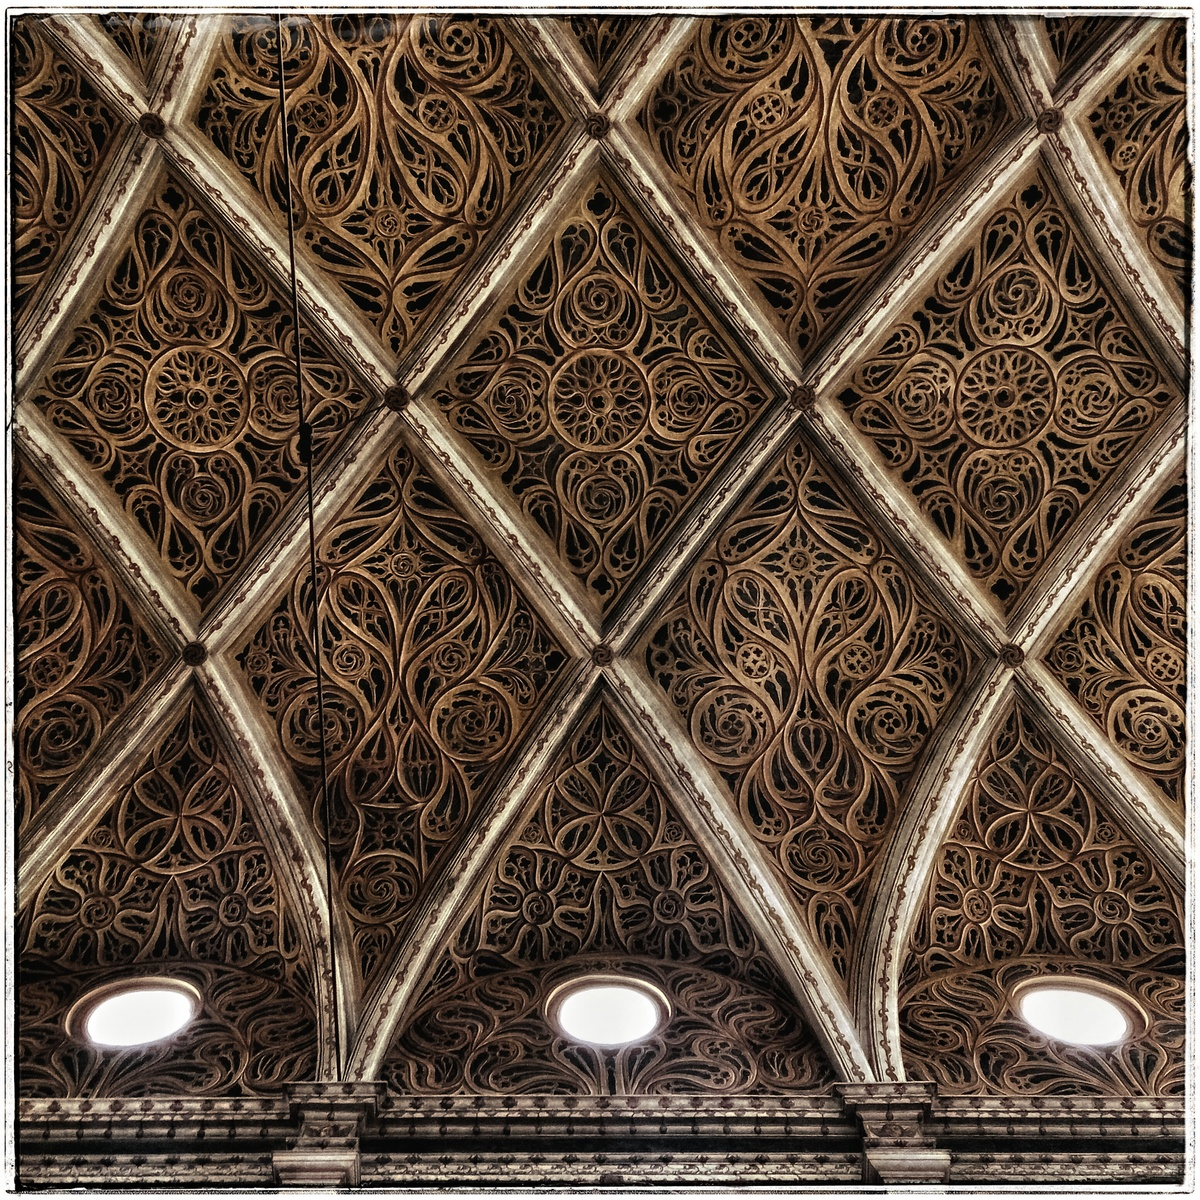
\includegraphics{thumb-lesson_XXI.jpeg}
  %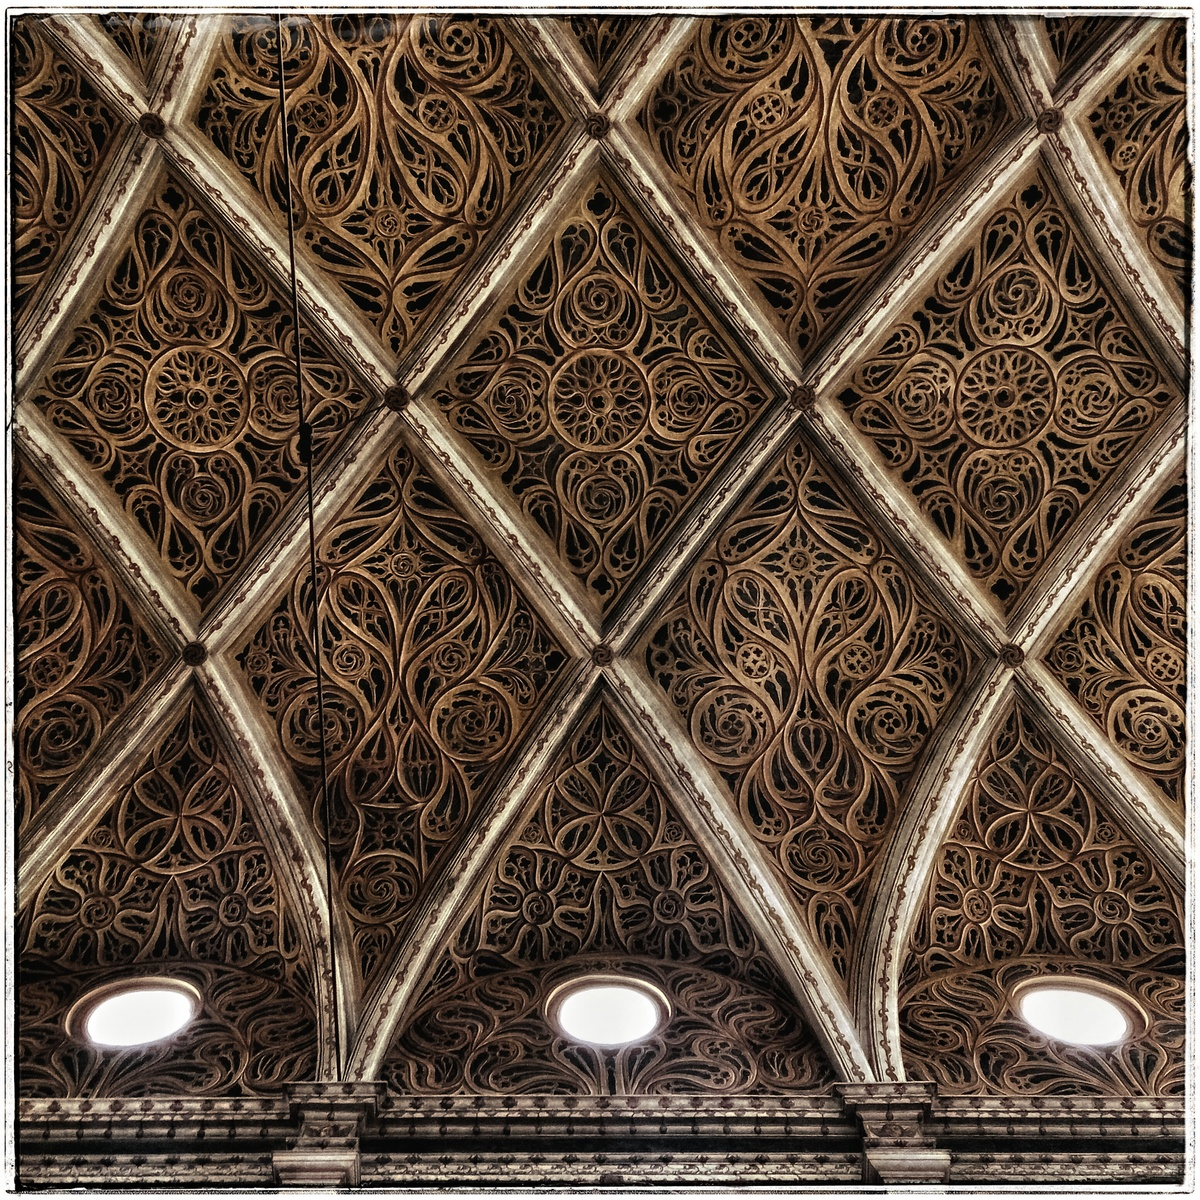
\includegraphics[width=0.9\linewidth]{thumb-lesson_XXI.jpeg}
  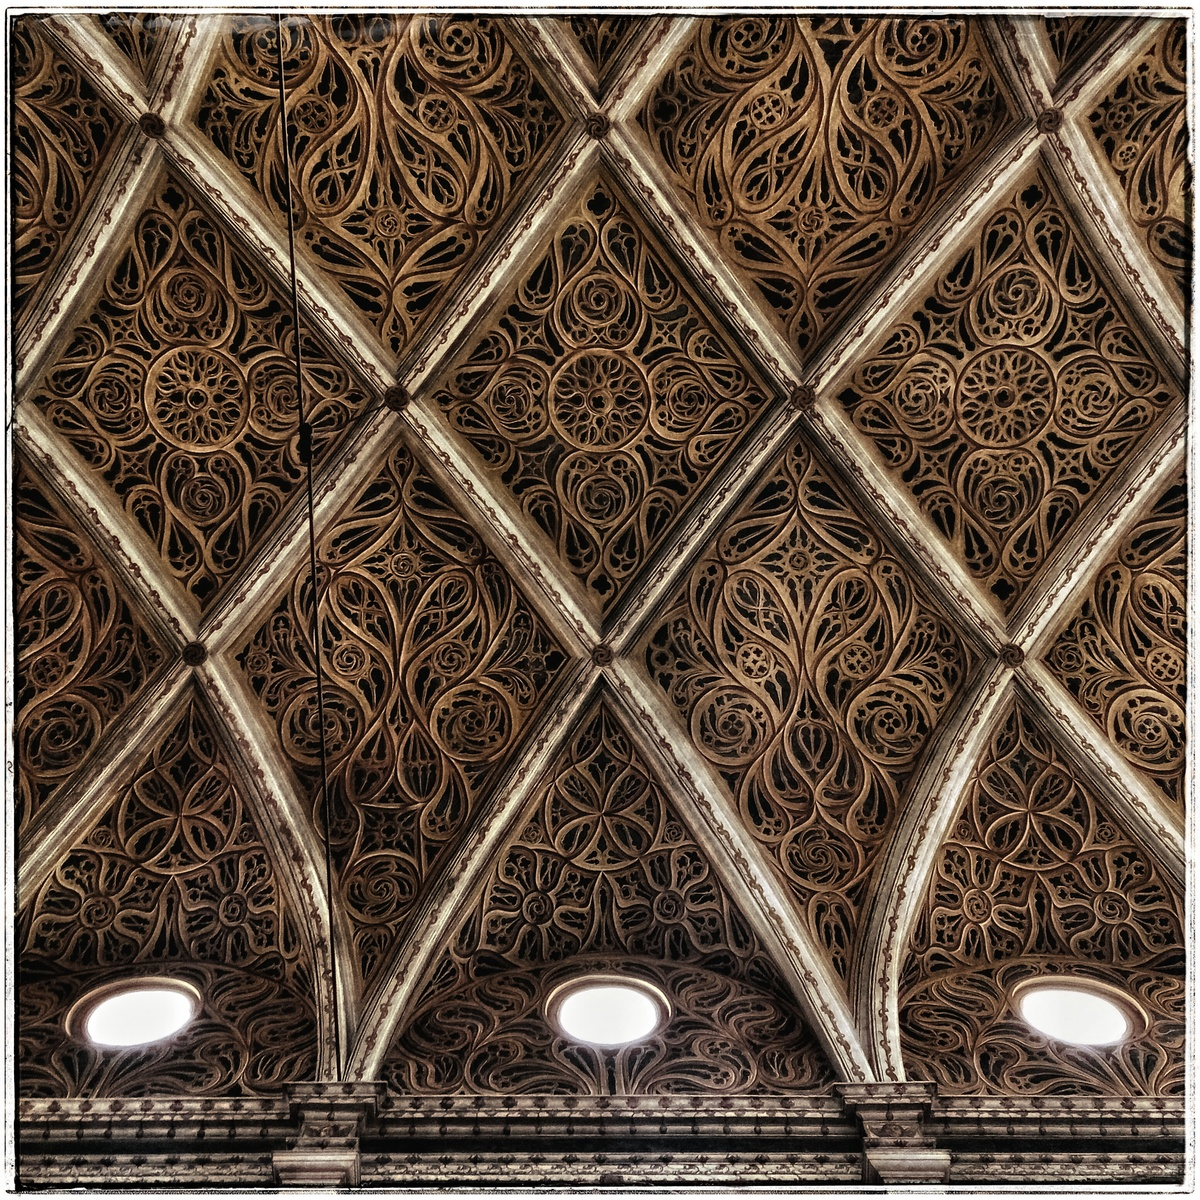
\includegraphics{thumb-lesson_XXI.jpeg}
  \caption{Milano: San Maurizio al Monastero Maggiore}
  \label{fig:textfig}
  %\zsavepos{pos:textfig}
  %\setfloatalignment{b}
\end{figure}

 

\nobibliography{latinBiblio}
\bibliographystyle{alpha}


\end{document}
